\documentclass{article}
\usepackage{caption}
\usepackage{subcaption}
\usepackage{graphicx}
\usepackage{tikz}
\usepackage{tikzsymbols}
\usetikzlibrary{calc,patterns,shapes.geometric}
\usepackage{float}
\usepackage{pdflscape}

\def\centerarc[#1](#2)(#3:#4:#5){\draw[#1] ($(#2)+({#5*cos(#3)},{#5*sin(#3)})$) arc (#3:#4:#5);}

\pagestyle{empty}
\begin{document}
	\centering
	\begin{figure}[H]
		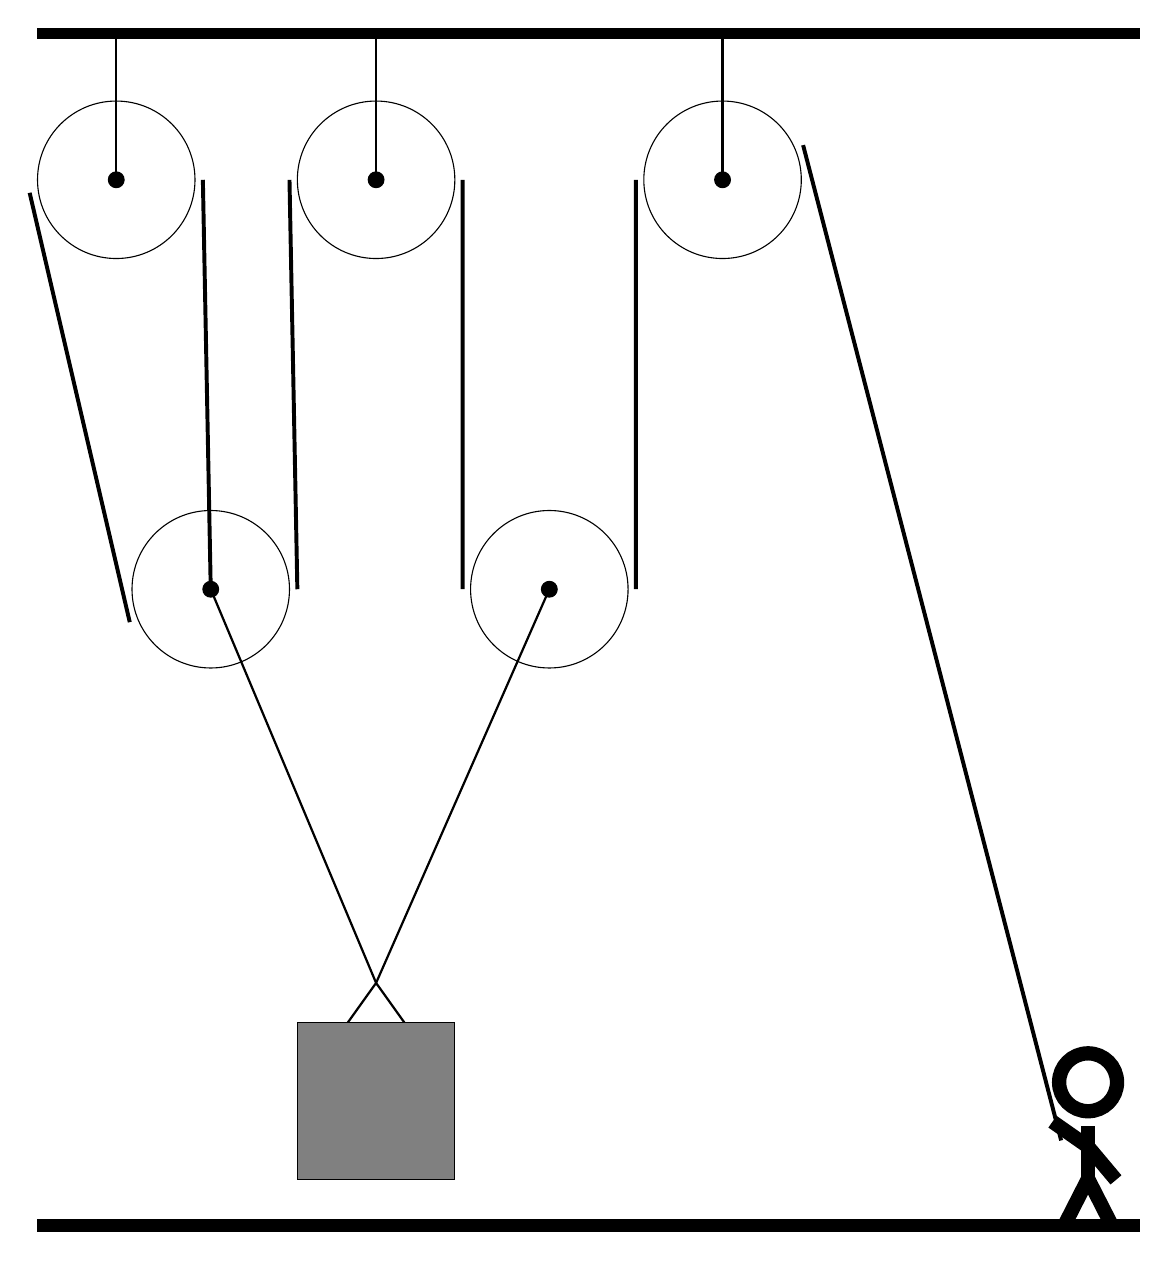
\begin{tikzpicture}
			%%%%% START %%%%%
			\def\a{12}
			\def\radlg{1}
			\def\radrp{1.1}
			\def\radsm{0.1}
			\def\yh{\a-0.15*\a}
			\def\yl{5}
			\def\xone{-1}
			\def\xtwo{2.3}
			\def\xthree{6.7}
			\def\xfour{0.2}
			\def\xfive{4.5}
			\def\dx{8.3}
			\def\dy{-1.9}
			\def\dw{1.75mm}
			\def\hlen{5}
			\def\width{0.5mm}
			\def\bump{0.3}
			
			\draw[fill=black] (-2,\a) rectangle (12,\a+0.125);
			
			\draw (\xone,\yh) circle (\radlg);
			\draw[fill=black] (\xone,\yh) circle (\radsm);
			\draw[thick] (\xone,\yh) -- (\xone,\a);
			
			\draw (\xtwo,\yh) circle (\radlg);
			\draw[fill=black] (\xtwo,\yh) circle (\radsm);
			\draw[thick] (\xtwo,\yh) -- (\xtwo,\a);
			
			\draw (\xthree,\yh) circle (\radlg);
			\draw[fill=black] (\xthree,\yh) circle (\radsm);
			\draw[thick] (\xthree,\yh) -- (\xthree,\a);
			
			\draw (\xfour,\yl) circle (\radlg);
			\draw[fill=black] (\xfour,\yl) circle (\radsm);	
			
			\draw (\xfive,\yl) circle (\radlg);
			\draw[fill=black] (\xfive,\yl) circle (\radsm);
			
			\draw[thick] (\xfour,\yl) -- (\xtwo,\yl-\hlen)  -- (\xfive,\yl);
			\draw[thick]  (\xtwo-0.5,\yl-\hlen-0.7) -- (\xtwo,\yl-\hlen) -- (\xtwo+0.5,\yl-\hlen-0.7);
			\draw[fill=black!50] (\xtwo-1,\yl-\hlen-0.5) rectangle (\xtwo+1,\yl-\hlen-2-0.5); 
			
			\draw[line width=\width] (\xfour,\yl) -- (\xone+\radrp,\yh); 
			\centerarc[line width=\width](\xone,\yh)(0:200:\radrp);
			\draw[line width=\width] (\xone-\radrp,\yh-\radrp*0.15) -- (\xfour-\radrp*0.935,\yl-0.38*\radrp); 
			\centerarc[line width=\width](\xfour,\yl)(200:360:\radrp);
			\draw[line width=\width](\xfour+\radrp,\yl) -- (\xtwo-\radrp,\yh); 
			\centerarc[line width=\width](\xtwo,\yh)(0:180:\radrp);
			\draw[line width=\width] (\xtwo+\radrp,\yh) -- (\xfive-\radrp,\yl); 
			\centerarc[line width=\width](\xfive,\yl)(180:360:\radrp);
			\draw[line width=\width] (\xfive+\radrp,\yl) -- (\xthree-\radrp,\yh);
			\centerarc[line width=\width](\xthree,\yh)(20:180:\radrp);
			\draw[line width=\width](\xthree+\radrp*0.93,\yh+0.4*\radrp)  -- (11, -2);
			
			\node at (11.3, -2) {\Strichmaxerl[10][-35][-50]};
			
			\draw[fill=black] (-2,-3) rectangle (12,-3.15);
			%%%%% END %%%%%
		\end{tikzpicture}
	\end{figure}
	
\end{document}